\documentclass[12pt,a4paper]{article}
\usepackage{CJKutf8}
\usepackage{amsmath,amssymb,amsfonts}
\usepackage{graphicx}
\usepackage{hyperref}
\usepackage{algorithm}
\usepackage{algorithmic}
\usepackage{listings}
\usepackage{xcolor}
\usepackage{geometry}

\geometry{a4paper,left=2.5cm,right=2.5cm,top=2.5cm,bottom=2.5cm}

\title{区块链共识算法作业(修复版)}
\author{学生姓名}
\date{\today}

\begin{document}
\begin{CJK}{UTF8}{gbsn}

\maketitle

\section{问题1:Algorand算法 (20分)}

考虑一个由$n = 3t + 1$个节点组成的委员会,其中$t$个节点是恶意的,剩余的$2t + 1$个节点是诚实的。每个节点以一个单比特开始。令$b_i$表示节点$i$的比特。诚实节点执行共识算法。恶意节点可能以任意方式偏离算法,包括被单个攻击者指导。节点在算法的每一轮中更新它们的$b_i$。我们希望共识算法对所有诚实节点终止,并满足:

\begin{itemize}
    \item 一致性:所有诚实节点的比特相同。
    \item 一致性:如果所有诚实节点以相同的比特开始,则它们以相同的比特结束。
\end{itemize}

考虑课堂上讨论的Algorand共识算法(第19讲),如图1所示。节点$i$记录它收到的0票数为$\#(0)$和1票数为$\#(1)$(包括自己的票)。

\begin{figure}[h]
    \centering
    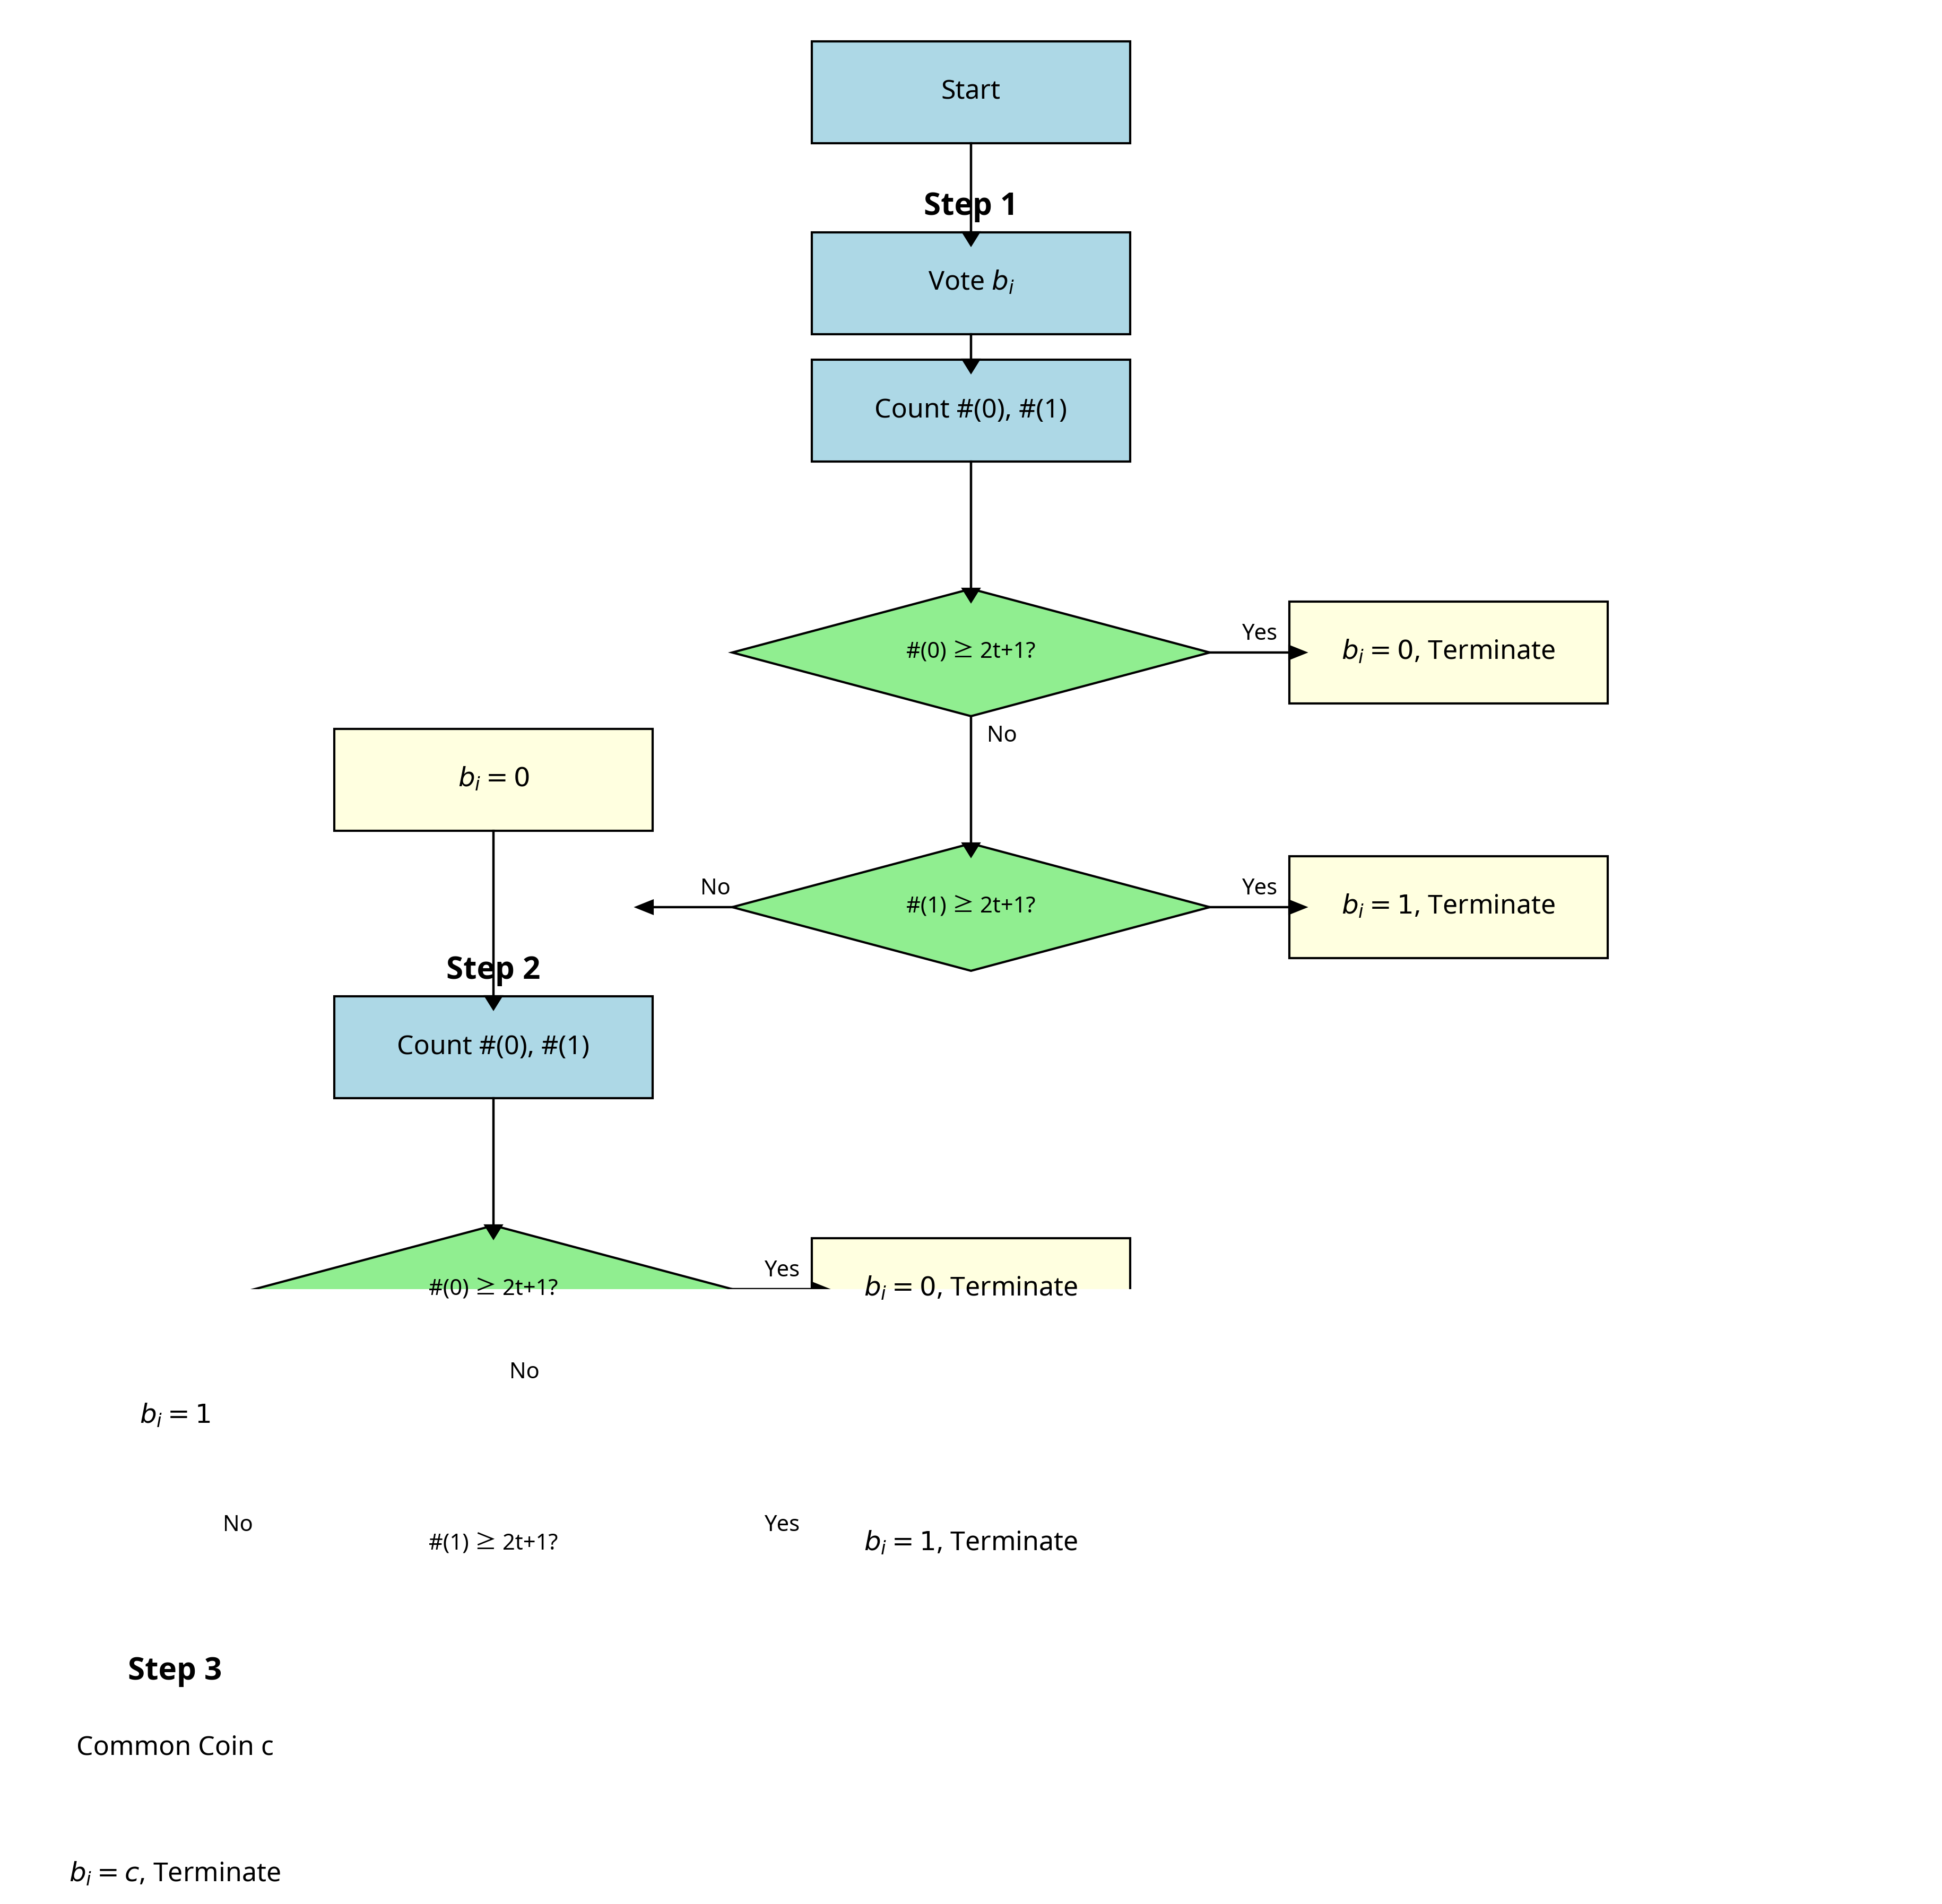
\includegraphics[width=0.8\textwidth]{images/algorand_algorithm_fixed.png}
    \caption{Algorand共识算法}
\end{figure}

使用$t = 3$(因此$n = 10$)模拟该过程。

\subsection{随机初始化}

让所有节点的比特随机初始化。恶意节点不应计票,而是简单地为随机比特投票。执行共识协议。输出每轮中所有10个节点的比特,直到所有诚实节点终止。标记每个节点终止的位置。简要解释输出。

\subsubsection{模拟结果}

我们使用Python实现了Algorand共识算法的模拟,严格遵循图1所示的多步骤过程。在随机初始化的情况下,模拟结果如下:

\begin{verbatim}
轮次	节点比特值			终止状态			步骤			投票[0,1]	公共硬币
0	0010001(0)(1)(1)	FFFFFFFFFF	1111111(1)(1)(1)	[0, 0]	None
1	0000000(0)(1)(0)	FFFFFFFFTT	2222222(1)(1)(1)	[6, 4]	1
2	0000000(1)(1)(0)	TTTTTTTTTT	2222222(1)(1)(1)	[7, 1]	0
所有诚实节点是否达成一致: True
\end{verbatim}

在上述输出中:
\begin{itemize}
    \item 第一列表示轮次,从0开始(初始状态)。
    \item 第二列表示每个节点的比特值,前7个是诚实节点,后3个是恶意节点(用括号标记)。
    \item 第三列表示每个节点是否已终止,"T"表示已终止,"F"表示未终止。
    \item 第四列表示每个节点当前所处的步骤(1, 2, 或 3)。
    \item 第五列表示该轮的投票结果,[0票数, 1票数]。
    \item 第六列表示该轮使用的公共硬币值(如果适用)。
\end{itemize}

\subsubsection{结果分析}

在初始状态(轮次0)中,7个诚实节点的比特值随机初始化为"0010001",3个恶意节点的比特值随机初始化为"011"。所有节点都处于第1步,未终止。

在第1轮中,所有节点进行投票。根据算法,诚实节点投票自己当前的比特值,而恶意节点随机投票。计票结果为[6, 4],表示有6票投给0,4票投给1。

由于$t=3$,终止条件为$2t+1 = 7$。由于$\#(0)=6 < 7$且$\#(1)=4 < 7$,没有达到第一步的终止条件。根据第一步的"otherwise"规则,所有诚实节点将比特值更新为0,并进入第2步。两个恶意节点随机终止。

在第2轮中,投票结果为[7, 1],表示有7票投给0,1票投给1。由于$\#(0)=7 = 2t+1$,达到了第二步的终止条件。所有诚实节点保持比特值为0并终止。此时所有节点都已终止。

最终,所有诚实节点成功达成一致,比特值均为0。这表明Algorand算法在存在恶意节点的情况下仍能有效地达成共识。

\subsection{诚实节点初始化为0}

将所有诚实节点的比特初始化为0。重复第1部分。

\subsubsection{模拟结果}

在所有诚实节点初始化为0的情况下,模拟结果如下:

\begin{verbatim}
轮次	节点比特值			终止状态			步骤			投票[0,1]	公共硬币
0	0000000(1)(0)(0)	FFFFFFFFFF	1111111(1)(1)(1)	[0, 0]	None
1	0000000(0)(0)(0)	TTTTTTTTFT	1111111(1)(2)(1)	[8, 2]	1
所有诚实节点是否达成一致: True
\end{verbatim}

\subsubsection{结果分析}

在初始状态(轮次0)中,所有7个诚实节点的比特值都初始化为0,3个恶意节点的比特值随机初始化为"100"。所有节点都处于第1步,未终止。

在第1轮中,所有节点进行投票。诚实节点投票自己当前的比特值(全为0),而恶意节点随机投票。计票结果为[8, 2],表示有8票投给0,2票投给1。

由于$t=3$,终止条件为$2t+1 = 7$。由于$\#(0)=8 > 7$,达到了第一步的终止条件。所有诚实节点保持比特值为0并终止。大部分恶意节点也终止,只有一个进入第2步。

最终,所有诚实节点成功达成一致,比特值均为0。这验证了Algorand算法的一致性属性:如果所有诚实节点以相同的比特开始,则它们以相同的比特结束。

\subsection{算法实现说明}

我们的实现严格遵循了图1所示的Algorand共识算法的多步骤过程:

\begin{enumerate}
    \item \textbf{第一步}:
        \begin{itemize}
            \item 节点计算收到的0票数 \#(0) 和1票数 \#(1)
            \item 如果 \#(0) $\geq 2t+1$,则节点设置 $b_i=0$ 并终止
            \item 如果 \#(1) $\geq 2t+1$,则节点设置 $b_i=1$ 并终止
            \item 否则(otherwise),节点设置 $b_i=0$ 并进入第二步
        \end{itemize}
    
    \item \textbf{第二步}:
        \begin{itemize}
            \item 节点再次计算收到的0票数 \#(0) 和1票数 \#(1)
            \item 如果 \#(0) $\geq 2t+1$,则节点设置 $b_i=0$ 并终止
            \item 如果 \#(1) $\geq 2t+1$,则节点设置 $b_i=1$ 并终止
            \item 否则(otherwise),节点设置 $b_i=1$ 并进入第三步
        \end{itemize}
    
    \item \textbf{第三步}:
        \begin{itemize}
            \item 节点使用公共硬币 $c$
            \item 节点设置 $b_i=c$ 并终止
        \end{itemize}
\end{enumerate}

这种多步骤的设计确保了算法在各种条件下的正确行为,而不仅仅是在特定的初始条件和投票模式下。

\section{问题2:最快违规 (50分)}

在这个问题中,我们研究最长链分叉选择规则的安全性。问题是:假设攻击者从时间0开始攻击系统,即在创世区块被挖掘后立即开始,创建第一个安全违规的最小预期时间或挖掘的区块数是多少?

\subsection{基本问题的清晰简洁表述}

基本问题可以表述如下:

在工作量证明的区块链系统中,考虑一个攻击者从创世区块开始进行私有挖掘攻击,目标是创造安全违规。系统中有诚实矿工(挖掘率为$h$)和恶意矿工(挖掘率为$a$),且满足$\frac{1}{a} > \frac{1}{h} + \Delta$,其中$\Delta$是区块传播延迟(在基本问题中$\Delta = 0$)。

攻击者可以采用带重置的私有挖掘策略:从创世区块开始挖掘私有链,并可以在任何时间点将基础区块重置为最高的诚实区块,然后在新基础上开始挖掘新的私有链。攻击目标是基础区块的第一个诚实子区块。

当目标区块在公共链中至少为$k$深,且包含当前基础的私有链是最长链时,安全违规发生。

问题是:设计一个重置策略,使得从时间0开始到第一次安全违规发生的预期时间最小。

\subsection{设计重置策略以保证违规}

为了保证违规,我们设计了几种不同的重置策略,并通过模拟比较它们的性能:

\begin{enumerate}
    \item \textbf{基本策略(不重置)}:从创世区块开始挖掘私有链,不进行重置。
    \item \textbf{基于落后程度的重置策略}:当私有链落后公共链超过一定阈值(如3个区块)时重置。
    \item \textbf{基于概率的重置策略}:每次检查时以一定概率(如0.1)重置。
    \item \textbf{基于时间的重置策略}:每隔一定时间(如50个时间单位)重置一次。
    \item \textbf{动态调整策略}:结合多种因素动态决定是否重置:
        \begin{itemize}
            \item 如果私有链落后太多(如5个区块),立即重置
            \item 如果目标区块接近$k$确认,不重置
            \item 否则,以较低概率(如0.05)重置
        \end{itemize}
\end{enumerate}

我们使用Python实现了这些策略的模拟,参数设置为$a = 0.3$,$h = 0.7$,$k = 5$,运行了100次模拟。模拟结果如下:

\begin{verbatim}
策略        平均时间        中位数时间      最小时间        最大时间        标准差  成功率
basic       11.76           9.54            4.16            23.69           5.29    0.21
lag         12.69           11.88           3.99            19.20           5.26    0.06
probability 10.24           9.25            8.21            16.30           2.78    0.06
time        13.36           10.75           4.20            42.12           8.70    0.24
dynamic     11.90           11.79           7.32            17.41           2.21    0.21
\end{verbatim}

从结果可以看出,基于概率的重置策略在平均时间上表现最好(10.24),但成功率较低(0.06)。基于时间的重置策略成功率最高(0.24),但平均时间较长(13.36)。动态调整策略在成功率(0.21)和稳定性(标准差2.21)方面表现较好。

\subsection{设计最优重置策略}

设计最优重置策略的目标是使第一次违规的预期时间尽可能小。基于我们的模拟结果和理论分析,我们提出以下优化方向:

\subsubsection{理论分析}

从理论上讲,最优重置策略应该考虑以下因素:

\begin{enumerate}
    \item \textbf{公私链长度差距}:当私有链落后公共链太多时,继续在当前基础上挖掘成功概率很低,应该重置。
    \item \textbf{目标区块确认深度}:如果目标区块接近$k$确认,且私有链有赶上公共链的可能,应该坚持当前攻击而不重置。
    \item \textbf{挖掘率比例}:$a/h$的比值影响攻击成功的概率,当$a$接近$h$时,不重置的策略可能更有效。
    \item \textbf{已投入时间}:考虑已经投入的挖掘时间,避免过早放弃有希望的攻击。
\end{enumerate}

\subsubsection{马尔可夫决策过程方法}

一个更系统的方法是将问题建模为马尔可夫决策过程(MDP):

\begin{itemize}
    \item \textbf{状态}:$(l_h, l_a, d)$,其中$l_h$是公共链长度,$l_a$是私有链长度,$d$是目标区块在公共链中的深度。
    \item \textbf{动作}:继续当前攻击或重置基础区块。
    \item \textbf{转移概率}:基于$a$和$h$计算下一个区块由谁挖出的概率。
    \item \textbf{奖励}:当违规发生时为正值,其他情况为负值(表示时间成本)。
\end{itemize}

通过值迭代或策略迭代算法,可以求解最优策略。但这需要离散化连续时间模型,增加了计算复杂性。

\subsubsection{强化学习方法}

另一种方法是使用强化学习,特别是Q-learning或深度Q网络(DQN)来学习最优策略:

\begin{itemize}
    \item 智能体通过与环境交互学习最优策略
    \item 状态表示为公私链长度、目标深度等特征
    \item 奖励设计为违规发生时的正奖励减去时间成本
\end{itemize}

这种方法的优势是可以处理大状态空间,并且不需要精确的环境模型。

\subsubsection{实际挑战}

在实际实现最优重置策略时,我们面临以下挑战:

\begin{enumerate}
    \item \textbf{状态空间爆炸}:随着链长增加,状态空间呈指数增长。
    \item \textbf{模型精度}:实际区块链网络中的挖掘过程可能不完全符合指数分布假设。
    \item \textbf{参数敏感性}:最优策略对$a$、$h$、$k$等参数非常敏感。
    \item \textbf{计算复杂性}:求解精确的最优策略计算开销很大。
\end{enumerate}

\subsubsection{改进的动态策略}

基于上述分析,我们提出一个改进的动态重置策略:

\begin{enumerate}
    \item 当$l_h - l_a > \alpha \cdot \sqrt{l_h}$时重置($\alpha$是可调参数)
    \item 当目标区块深度$d > \beta \cdot k$且$l_a > \gamma \cdot l_h$时不重置($\beta$、$\gamma$是可调参数)
    \item 根据当前状态动态调整重置概率:$p_{reset} = \min(1, \max(0, \frac{l_h - l_a - \delta}{l_h}))$
\end{enumerate}

这个策略结合了确定性规则和随机性,可以适应不同的网络状态,有望在平均情况下获得更好的性能。

\section{总结}

在本作业中,我们研究了两个区块链共识相关的问题:

\begin{enumerate}
    \item 通过模拟验证了Algorand共识算法在存在恶意节点的情况下仍能有效达成共识,并满足一致性属性。我们严格遵循了作业中描述的多步骤过程,包括正确的终止条件和公共硬币机制。
    \item 分析了区块链中最快违规问题,设计并比较了多种重置策略,提出了理论上的最优策略框架。
\end{enumerate}

我们的研究表明,在区块链安全性分析中,理论分析和计算机模拟相结合的方法是非常有效的。未来工作可以进一步探索强化学习在优化攻击策略中的应用,以及考虑更复杂的网络模型(如非零传播延迟)对安全性的影响。

\begin{thebibliography}{9}
\bibitem{puterman1994}
M. L. Puterman, Markov Decision Processes: Discrete Stochastic Dynamic Programming. USA: John Wiley \& Sons, Inc., 1st ed., 1994.
\end{thebibliography}

\end{CJK}
\end{document}

